\begin{center}
  \scalebox{0.68}{
    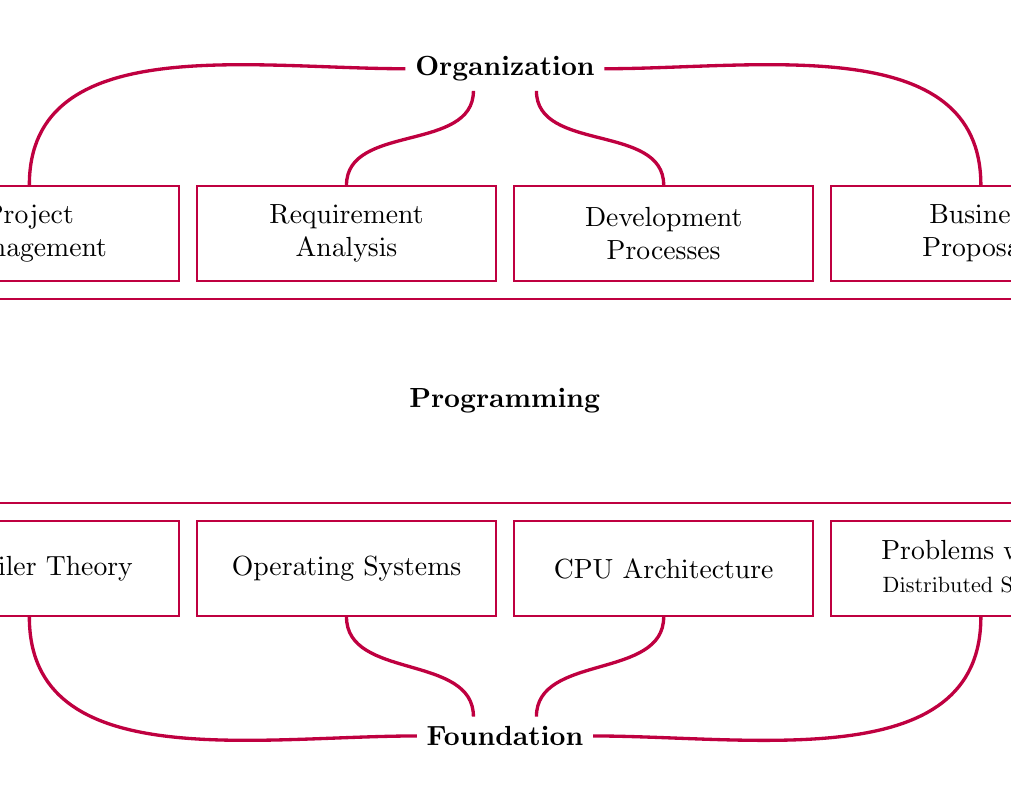
\begin{tikzpicture}[remember picture]
      \newcommand{\blockwidth}[0]{3.8cm}
      \newcommand{\width}[0]{(4*\blockwidth+3*2mm)}
      \newcommand{\ewidth}[0]{(\width+0.8mm)}
      \newcommand{\height}[0]{9cm}
      \newcommand{\xoffset}[0]{6mm}
      
      \coordinate (origo) at (\xoffset,-\height);
      
      \tikzstyle{node}=[
        overlay,
        rectangle,
        draw=purple,
        anchor=center,
        align=center,
        thick,
        minimum width=\blockwidth,
        minimum height=1.2cm,
      ]
      \tikzstyle{title} = [
        anchor=south,
        align=center,
      ]
      \tikzstyle{edge}  = [
        very thick,
        >=stealth,
        draw=purple,
      ]
      
      % organization
      \node[label, anchor=north] (organization) at ([xshift=\ewidth/2] \xoffset,0) {\textbf{Organization}};
      
      % programming
      \node[node, anchor=center, minimum height=2.6cm,minimum width=\ewidth]
        (programming) at ({\xoffset+\ewidth/2}, -\height/2]) {\textbf{Programming}};
      
      % foundation
      \node[label, anchor=south] (foundation) at ([xshift=\ewidth/2] origo) {\textbf{Foundation}};
      
      % CS boxes
      {
        \node[node, anchor=north west]
          (compiler) at ([yshift=-2mm] programming.south west) {Compiler Theory};
        \draw[edge] (compiler.south) to [out=270,in=180] (foundation.west);
      }
      {
        \node[node, anchor=north west]
          (os) at ([xshift=2mm] compiler.north east) {Operating Systems};
        \draw[edge] (os.south) to [out=270,in=90] ([xshift=-4mm] foundation.north);
      }
      {
        \node[node, anchor=north west]
          (cpu) at ([xshift=2mm] os.north east) {CPU Architecture};
        \draw[edge] (cpu.south) to [out=270,in=90] ([xshift=4mm] foundation.north);
      }
      {
        \node[node, anchor=north west]
          (dist) at ([xshift=2mm] cpu.north east) {Problems within\\\scalebox{0.8}{Distributed Systems}};
        \draw[edge] (dist.south) to [out=270,in=0] (foundation.east);
      }
      
      % SE boxes
      {
        \node[node, anchor=south west]
          (pm) at ([yshift=2mm] programming.north west) {Project\\Management};
        \draw[edge] (pm.north) to [out=90,in=180] (organization.west);
      }
      {
        \node[node, anchor=south west]
          (reqs) at ([xshift=2mm] pm.south east) {Requirement\\Analysis};
        \draw[edge] (reqs.north) to [out=90,in=270] ([xshift=-4mm] organization.south);
      }
      {
        \node[node, anchor=south west]
          (devp) at ([xshift=2mm] reqs.south east) {Development\\Processes};
        \draw[edge] (devp.north) to [out=90,in=270] ([xshift=4mm] organization.south);
      }
      {
        \node[node, anchor=south west]
          (business) at ([xshift=2mm] devp.south east) {Business\\Proposals};
        \draw[edge] (business.north) to [out=90,in=0] (organization.east);
      }
      
      % CS
      {
        \draw[overlay,decorate,decoration={brace, mirror, amplitude=10pt, raise=5pt}] ([xshift=0mm] programming.north west) to node[black,midway,left=15pt] {\rotatebox{90}{Computer Science}} ([xshift=0mm] compiler.south west);
      }
      
      % SE
      {
        \draw[overlay,decorate,decoration={brace, mirror, amplitude=10pt, raise=5pt}] ([xshift=0mm, yshift=2mm] dist.north east) to node[black,midway,right=15pt] {\rotatebox{90}{Software Engineering}} ([xshift=0mm] business.north east);
      }
    \end{tikzpicture}
  }
\end{center}
